\ifdefined\animada
\documentclass[aspectratio=169,11pt]{beamer}
\else
\documentclass[aspectratio=169,11pt,handout]{beamer}
\fi
\let\originalpercent\%
\usepackage[spanish,es-nodecimaldot]{babel}
\AtBeginDocument{\let\%\originalpercent}
\usepackage{booktabs,tabularx,amsmath,graphicx}
\graphicspath{{../../img/}}
% Identidad: Manual resumido de marca CUC, edición publicada en agosto de 2024.
% Logo vectorial oficial, sin reconstrucción ni modificación de sus elementos.
\usepackage{fontspec}
\usepackage{unicode-math}
\setmathfont{Latin Modern Math}
\defaultfontfeatures{Ligatures=TeX}
\setmainfont{RedHatDisplay}[Path=fuentes/,Extension=.ttf,UprightFont=*-Regular,BoldFont=*-Bold,ItalicFont=*-Italic]
\setsansfont{RedHatDisplay}[Path=fuentes/,Extension=.ttf,UprightFont=*-Regular,BoldFont=*-Bold,ItalicFont=*-Italic]
\definecolor{cucrojo}{HTML}{A3161A}
\definecolor{cucoro}{HTML}{C9A227}
\definecolor{cucgris}{HTML}{595959}
\definecolor{cucplata}{HTML}{CCCCCC}
\newcommand{\logocuc}[1]{
\includegraphics[width=#1]{marca/cuc-logo-vector.pdf}}

\usefonttheme{professionalfonts}
\definecolor{tinta}{HTML}{292929}\definecolor{acento}{HTML}{A3161A}\definecolor{gris}{HTML}{595959}
\setbeamercolor{normal text}{fg=tinta,bg=white}\setbeamercolor{structure}{fg=acento}
\setbeamercolor{frametitle}{fg=tinta}\setbeamerfont{frametitle}{size=\Large,series=\bfseries}
\setbeamertemplate{navigation symbols}{}\setbeamersize{text margin left=9mm,text margin right=9mm}
\setbeamertemplate{itemize item}{\small\textbullet}
\setbeamertemplate{footline}{%
\hspace{9mm}\begin{minipage}[c]{30mm}\logocuc{29mm}\end{minipage}%
\hfill\textcolor{cucgris}{\tiny ELECTRÓNICA II · FASE 2}\hfill%
\textcolor{cucrojo}{\scriptsize\insertframenumber\,/\,\inserttotalframenumber}\hspace{9mm}\vspace{3mm}}
\setbeamertemplate{frametitle}{\vspace{4mm}\insertframetitle\par\vspace{2mm}\textcolor{cucrojo}{\rule{\linewidth}{1pt}}}
\ifdefined\animada
  \addtobeamertemplate{background canvas}{}{\transfade[duration=0.35]}
\fi
\setbeamercovered{invisible}
\hypersetup{colorlinks=true,urlcolor=acento}
\ifdefined\connotas\setbeameroption{show notes on second screen=right}\fi
\begin{document}
\begin{frame}[t]{Filtros de audio: demostración de laboratorio}
\begin{columns}[T]\begin{column}{.43\textwidth}\vspace{1mm}\logocuc{57mm}\par\vspace{6mm}{\Large Analizador de espectro\par}\vspace{5mm}Leo Rojas\\David Orozco\\Manuel Castilla\par\vspace{5mm}\small Electrónica II · Universidad de la Costa\\Fase 2 · 22 de octubre de 2026\end{column}\begin{column}{.54\textwidth}\centering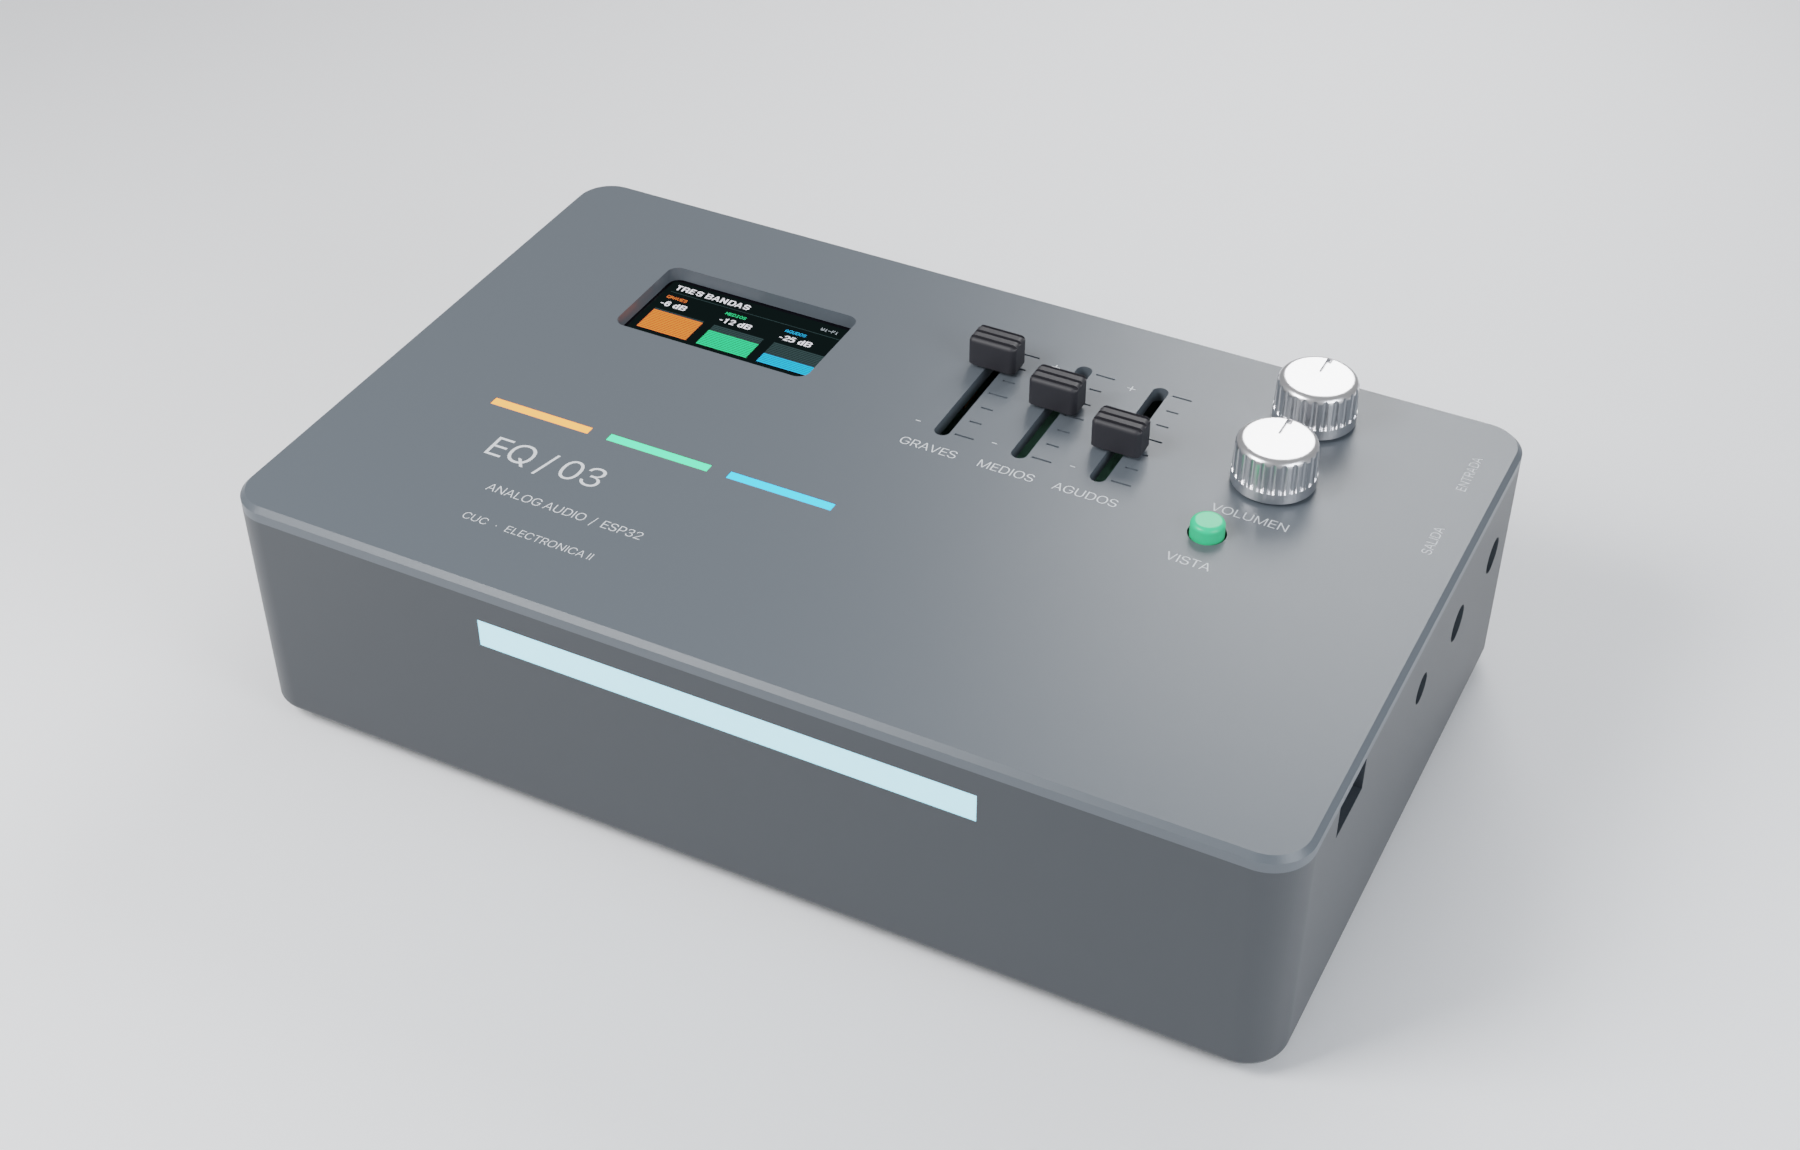
\includegraphics[width=\linewidth,height=5cm,keepaspectratio]{3d-gabinete-cerrado.png}\end{column}\end{columns}
\note{Este es el diseño del ecualizador: el audio pasa por filtros analógicos y el ESP32 muestra sus niveles y espectro. La imagen corresponde al modelo CAD.}
\end{frame}
\begin{frame}[t]{3,3 V de alimentación; 1,65 V de referencia}
\begin{columns}[T]\begin{column}{.66\textwidth}
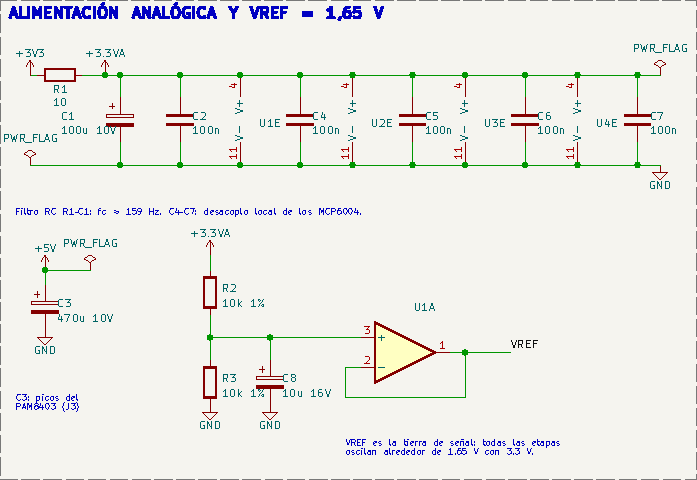
\includegraphics[width=\linewidth,height=4.9cm,keepaspectratio]{circuitos/referencia.pdf}
\end{column}\begin{column}{.30\textwidth}\small
R2 y R3 dividen la alimentación. U1A entrega VREF a los filtros.\par\vspace{4mm}
Filtro RC: R1 y C1.\par Desacoplo: C2 y C4–C7.\par\vspace{4mm}
En reposo: 1,641 V simulados.\par\vspace{4mm}
LED y alimentación del PAM8403: retorno a GND. El parlante va entre las dos salidas BTL.
\end{column}\end{columns}
\note{El audio oscila alrededor de VREF porque usamos una alimentación de 3,3 V. U1A evita cargar directamente el divisor. La caída en R1 deja la referencia en 1,641 V en la simulación. U1E es la unidad de alimentación de U1, no otro operacional. PWR\_FLAG es una marca para ERC; no se compra.}
\end{frame}
\begin{frame}[t]{Filtro de graves: U1C, R9, R10, C11 y C12}
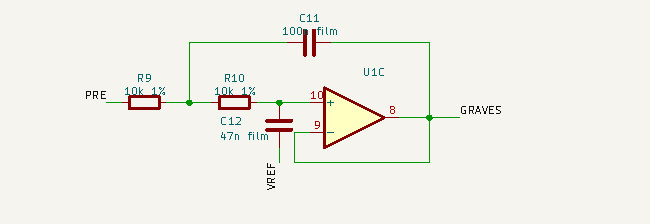
\includegraphics[width=.86\linewidth,height=3.3cm,keepaspectratio]{circuitos/graves.pdf}\par\vspace{3mm}
\begin{columns}[T]\begin{column}{.48\textwidth}\small
R9 = R10 = 10 k$\Omega$.\par C11 = 100 nF; C12 = 47 nF.\par U1C trabaja como seguidor.\end{column}\begin{column}<2->{.48\textwidth}\small
C11 vuelve desde la salida al nodo intermedio. C12 deriva a VREF.\par La realimentación fija $Q\approx0,73$; el corte simulado es 239 Hz.
\end{column}\end{columns}
\note{A baja frecuencia los condensadores cargan poco la señal; a alta frecuencia aumenta su efecto y cae la salida de graves. El filtro no es solo dos RC independientes: C11 realimenta desde la salida. Medios encadena pasa altas y pasa bajas; agudos usa pasa altas.}
\end{frame}
\begin{frame}[t]{Medios: dos filtros conectados en cascada}
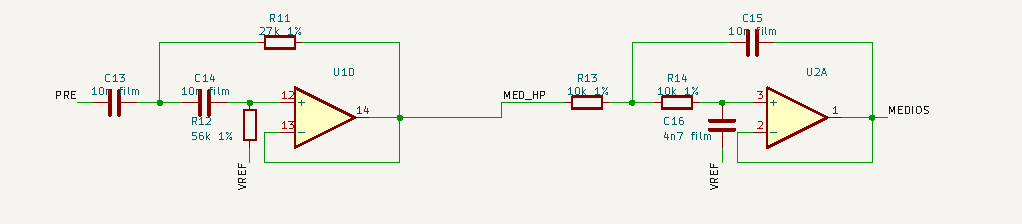
\includegraphics[width=\linewidth,height=3.1cm,keepaspectratio]{circuitos/medios.pdf}\par\vspace{4mm}
\begin{columns}[T]\begin{column}{.48\textwidth}\small
U1D: pasa altas de 403 Hz.\par C13 = C14 = 10 nF.\par R11 = 27 k$\Omega$; R12 = 56 k$\Omega$.
\end{column}\begin{column}<2->{.48\textwidth}\small
U2A: pasa bajas de 2388 Hz.\par R13 = R14 = 10 k$\Omega$.\par C15 = 10 nF; C16 = 4,7 nF.
\end{column}\end{columns}
\note{La salida de U1D entra directamente a U2A por MED\_HP. El primer filtro atenúa los graves y el segundo atenúa los agudos. Entre ambos queda la banda de medios. Son dos secciones de segundo orden conectadas en cascada.}
\end{frame}
\begin{frame}[t]{Agudos: pasa altas con U2B}
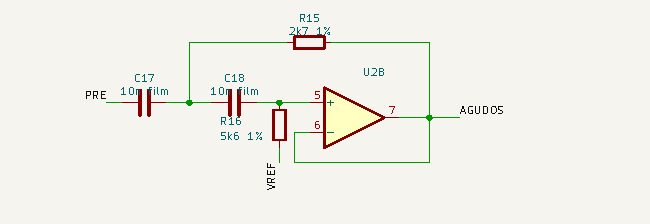
\includegraphics[width=.88\linewidth,height=3.4cm,keepaspectratio]{circuitos/agudos.pdf}\par\vspace{3mm}
\begin{columns}[T]\begin{column}{.48\textwidth}\small
C17 = C18 = 10 nF.\par R15 = 2,7 k$\Omega$; R16 = 5,6 k$\Omega$.
\end{column}\begin{column}<2->{.48\textwidth}\small
Corte simulado: 4026 Hz.\par La salida llega a RV4, que regula su aporte a la mezcla.
\end{column}\end{columns}
\note{Los condensadores están en serie con la señal. A baja frecuencia atenúan la entrada; por encima del corte aumenta la salida de agudos. U2B trabaja como seguidor dentro del filtro.}
\end{frame}
\begin{frame}[t]{Frecuencias calculadas y simuladas}
\begin{center}\begin{tabular}{lrr}\toprule
Filtro & Cálculo de $f_0$ & Corte simulado\\\midrule
Graves (U1C), pasa bajas & 232 Hz & 239 Hz\\
Medios (U1D), pasa altas & 409 Hz & 403 Hz\\
Medios (U2A), pasa bajas & 2322 Hz & 2388 Hz\\
Agudos (U2B), pasa altas & 4093 Hz & 4026 Hz\\
Previo al ADC (U2D) & 4949 Hz & 5101 Hz\\\bottomrule\end{tabular}\end{center}\vspace{3mm}\[ f_{0,PB}=\frac{1}{2\pi R\sqrt{C_1C_2}}\qquad f_{0,PA}=\frac{1}{2\pi C\sqrt{R_1R_2}}\]\small Cada sección es de segundo orden. La cascada de medios es de cuarto orden.
\note{Distinguir frecuencia natural y corte a menos tres decibelios: con Q cercano a 0,73 no coinciden exactamente. Todos los cortes nominales simulados cumplen el margen del diez por ciento.}
\end{frame}
\begin{frame}[t]{Ensayo de hoy: generador y osciloscopio}
\begin{columns}[T]\begin{column}{.46\textwidth}
\textbf{Entrada PRE}\par Senoidal de 200 mV pico a pico.\par Offset: 1,65 V.\par\vspace{3mm}
CH1: PRE. CH2: salida del filtro.\par Masas al GND del circuito.\par\vspace{3mm}
100 Hz: graves.\par 1 kHz: medios.\par 8 kHz: agudos.
\end{column}\begin{column}{.50\textwidth}
\textbf{Qué explicar}\par Comparar amplitud y fase.\par $|H|=V_{pp,out}/V_{pp,in}$.\par\vspace{3mm}
En Velxio: clic derecho sobre el cable y \textit{Add to scope}.\par\vspace{3mm}\small Los operacionales de esta prueba son ideales. El ensayo físico debe usar el MCP6004 y alimentación de 3,3 V.
\end{column}\end{columns}
\note{Cargar filtros-1000Hz.vlx. El generador inyecta directamente en PRE; esta prueba aísla los filtros. Añadir PRE y la salida al osciloscopio. En el banco, no conectar la pinza de masa a VREF. Cambiar a 100 Hz y a 8 kHz para comparar las bandas.}
\end{frame}
\begin{frame}[t]{Velxio: tres tonos, tres bandas}
\begin{columns}[T]\begin{column}{.34\textwidth}
\textbf{Ejecutado en el navegador}\par\vspace{3mm}
100 Hz: graves.\par1 kHz: medios.\par8 kHz: agudos.\par\vspace{4mm}
Tres archivos \texttt{.vlx}\par con el motor SPICE activo.\par\vspace{4mm}\small Modelo de operacional ideal. Prueba de selectividad; no del equipo completo.
\end{column}\begin{column}{.63\textwidth}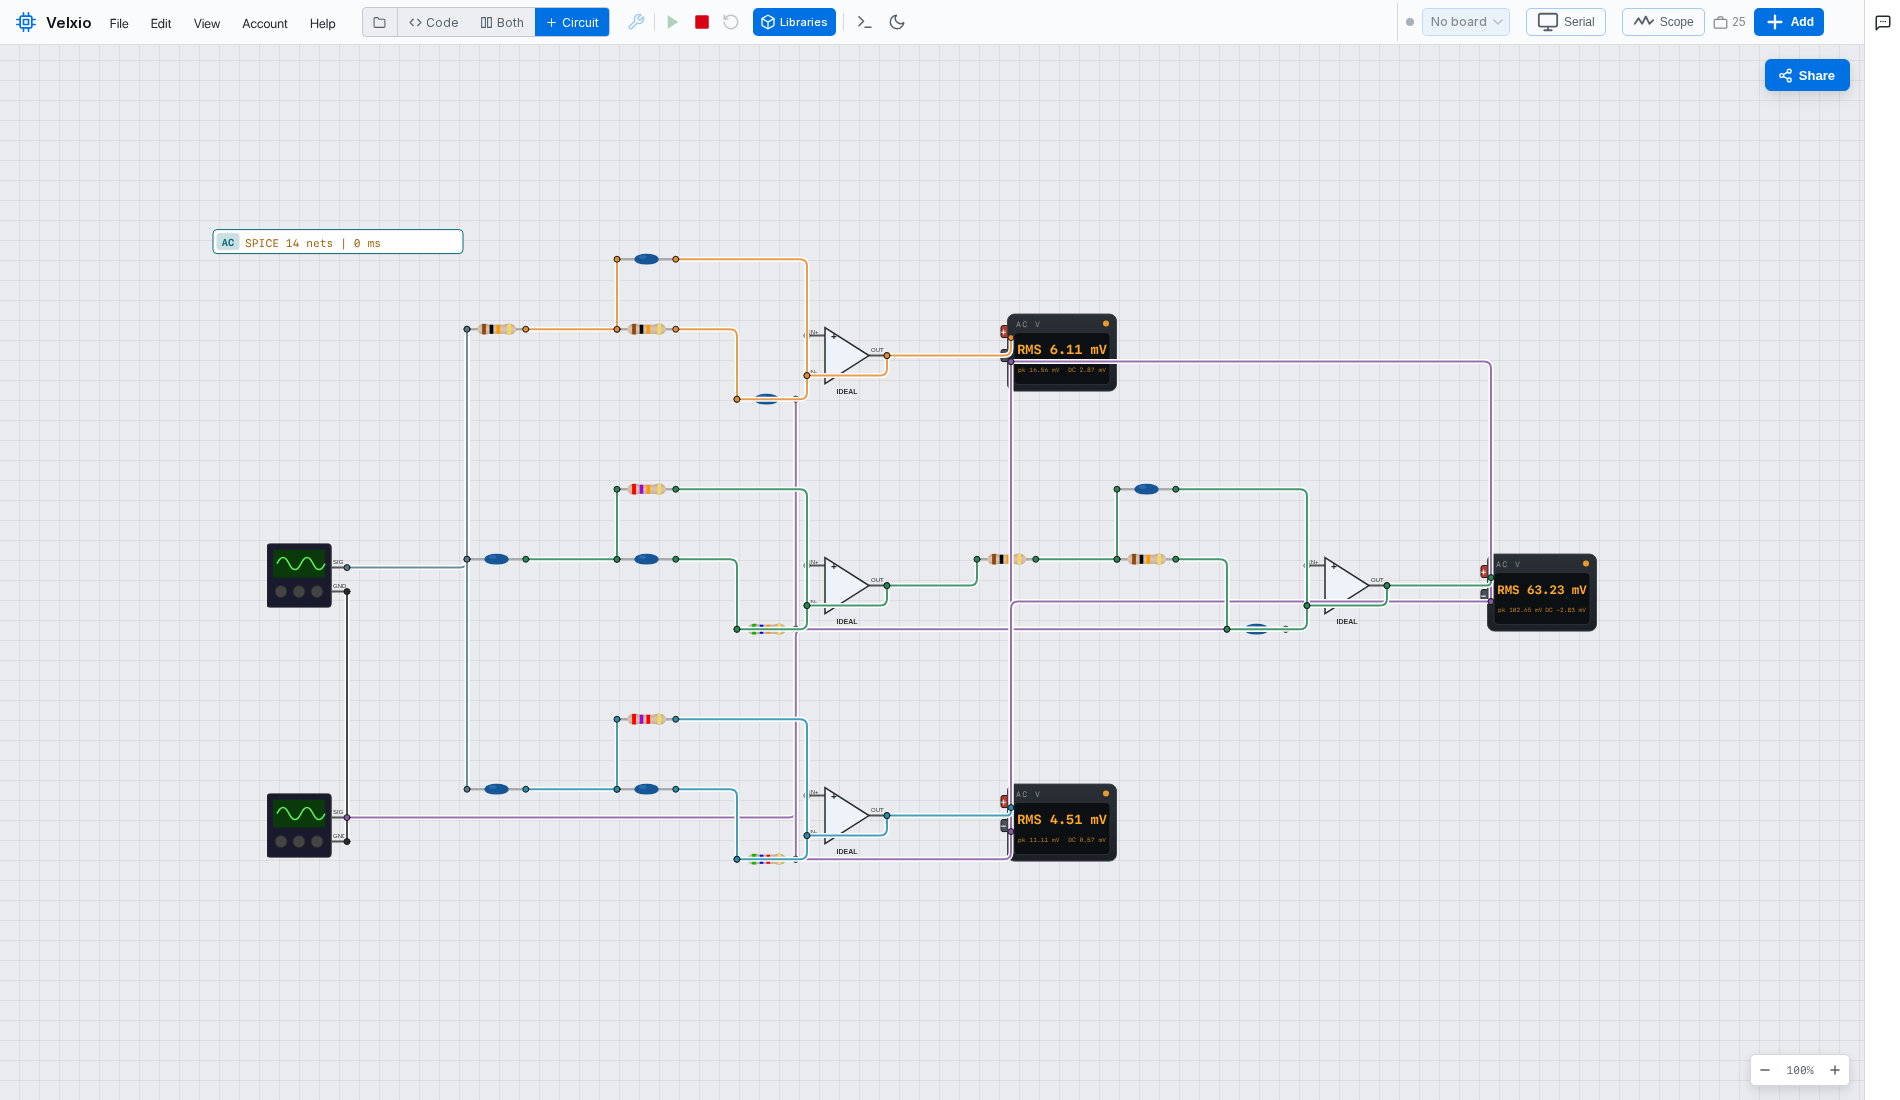
\includegraphics[width=\linewidth]{velxio-1000Hz.png}\end{column}\end{columns}
\note{Abrir File / Import project en Velxio y cargar uno de los tres archivos. Las lecturas RMS incluyen la ventana transitoria del simulador. En 1 kHz, medios registra 63,23 mV frente a 6,11 mV de graves y 4,51 mV de agudos. No atribuir al modelo ideal las limitaciones del MCP6004.}
\end{frame}
\begin{frame}[t]{Entrada y salida de medios en el osciloscopio}
\centering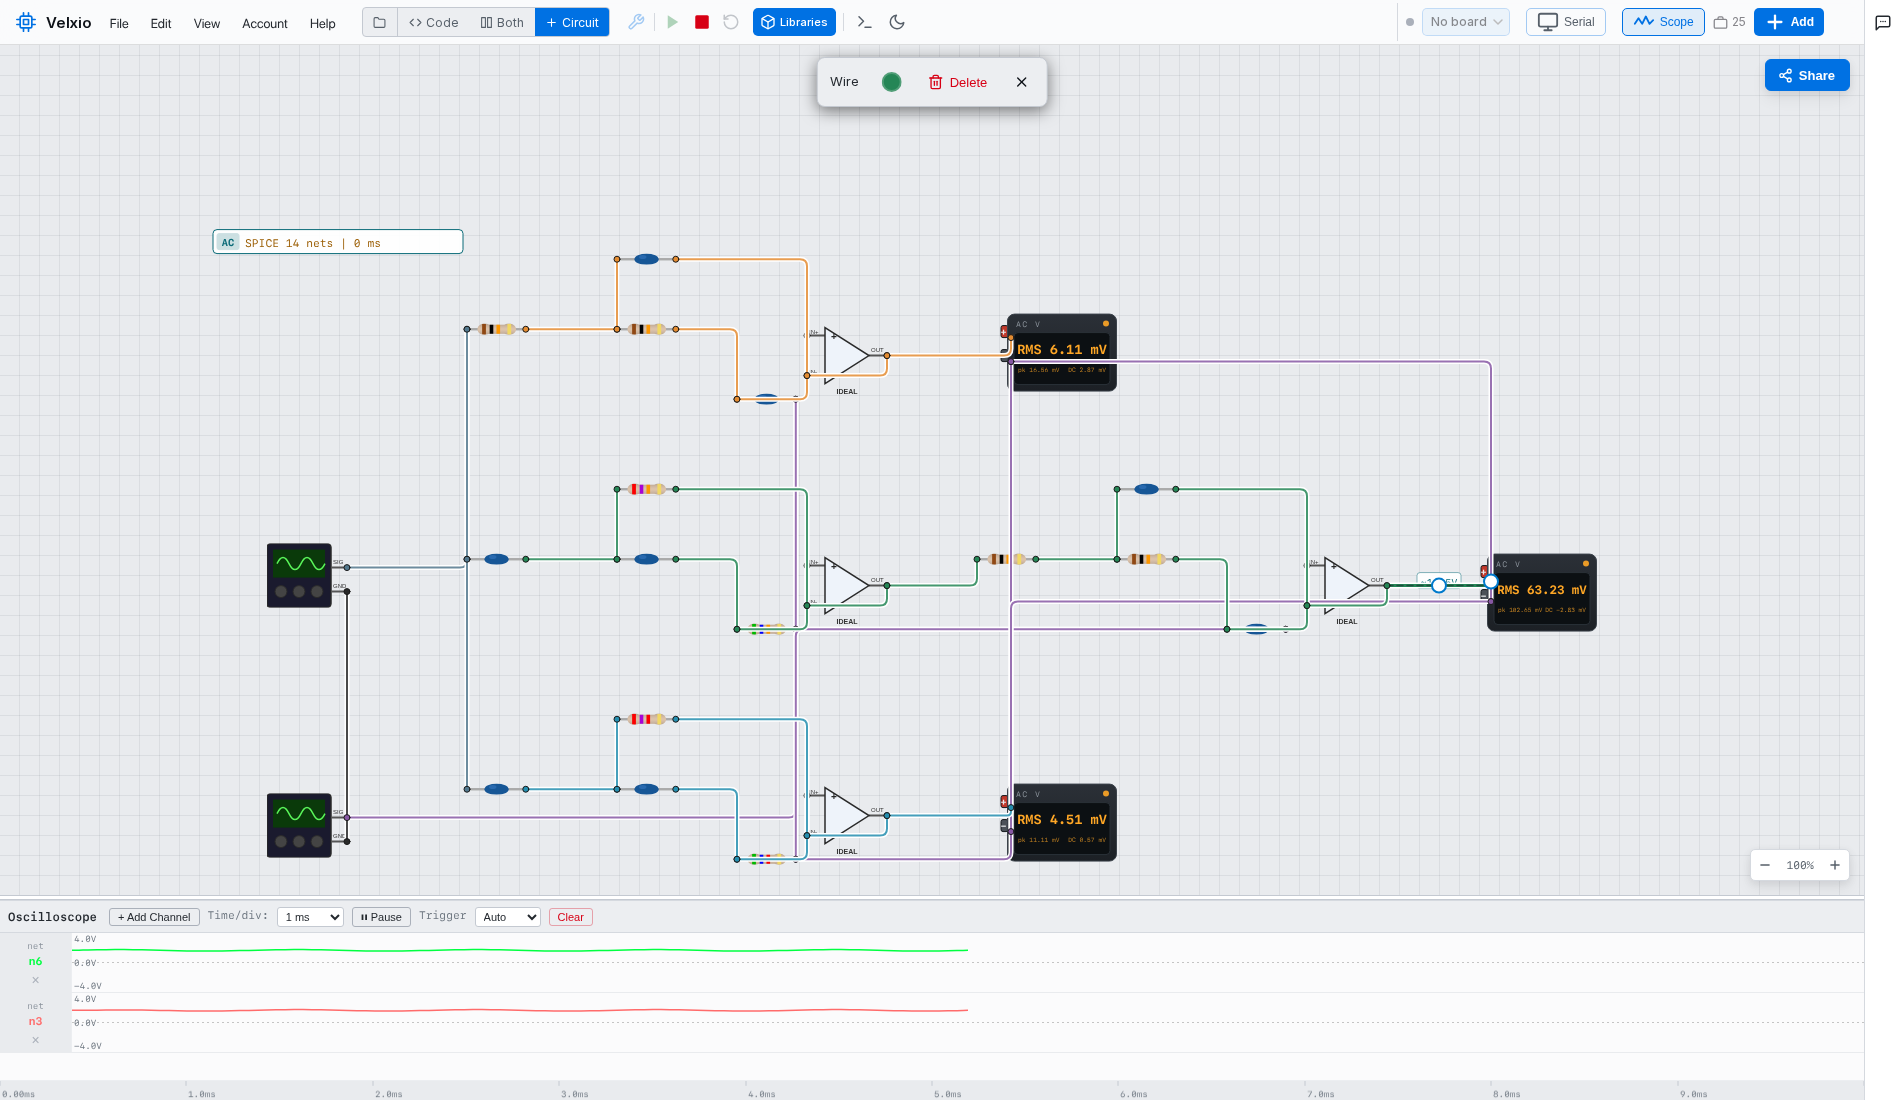
\includegraphics[width=\linewidth,height=5.5cm,keepaspectratio]{velxio-osciloscopio.png}
\note{Las sondas están en PRE y en la salida de medios. Es una captura del motor SPICE de Velxio, no una fotografía del osciloscopio del laboratorio. Comparar amplitud y desplazamiento temporal.}
\end{frame}
\begin{frame}[t]{Abrir la simulación durante la exposición}
\begin{columns}[T]\begin{column}{.65\textwidth}
\href{https://velxio.dev/editor?esp32sim=qemu}{\beamergotobutton{ABRIR VELXIO}}
\par\vspace{5mm}\url{https://velxio.dev/editor?esp32sim=qemu}\par\vspace{5mm}
\small Descargar un caso y usar \textbf{File $\rightarrow$ Import project}.\par\vspace{3mm}
100 Hz $\rightarrow$ graves\par 1 kHz $\rightarrow$ medios\par 8 kHz $\rightarrow$ agudos\par Ensayo LED $\rightarrow$ pulsar Run\par\vspace{4mm}
\href{run:../../simulacion/velxio/index.html}{\beamergotobutton{Abrir carpeta de casos}}
\par\vspace{3mm}\footnotesize Los casos .vlx también van adjuntos al PDF.
\end{column}\begin{column}{.29\textwidth}
\includegraphics[width=\linewidth]{velxio-qr.png}\par\small QR: abre el editor.\par Importar después el caso.
\end{column}\end{columns}
\note{El enlace y el QR abren Velxio; no abren automáticamente un proyecto publicado. Los archivos están en simulacion/velxio y adjuntos al PDF. Tener el caso de 1 kHz descargado antes de la exposición. El visor PDF puede bloquear enlaces a archivos locales; en ese caso abrir index.html desde la carpeta del proyecto.}
\end{frame}
\end{document}
